\section{Einleitung}
Es gibt viele Einflüsse die eine Auswirkung das Leben eines Menschen haben.
Es gibt jedoch vier Faktoren welche erhebliche Auswirkungen auf uns haben.

\begin{figurewrapper}
  \begin{tikzpicture}[small mindmap, concept color=gray!50, font=\sf, text=white,scale=1.5]
	\node[concept] {Person}
      child[concept color=\usedcolor, grow=0]{ node[concept,scale=1.5]{Soziale- und Kulturelle Verhältnisse}}
      child[concept color=\usedcolor, grow=60]{ node[concept,scale=1.5]{Geologische geografische Verhältnisse}}
      child[concept color=\usedcolor, grow=120]{ node[concept,scale=1.5]{Klima"-tische Verhältnisse}}
      child[concept color=\usedcolor, grow=180]{ node[concept,scale=1.5]{Politische Verhältnisse}};
  \end{tikzpicture}
  \captionof{figure}{Mindmap: Beeinflussende Faktoren einer Person}
\end{figurewrapper}

Soziale und Kulturelle Verhältnisse sind wichtig für das ganze Zwischenmenschliche.
Dies hat Auswirkungen auf die Lebensqualität  einer Person.

Politischen Verhältnisse beeinflussen jeden Menschen im Alltag,
denn in der Politik werden wichtige Entscheidungen getroffen,
die sich auf die Bewohner des jeweiligen Landes Auswirken.

Diese zwei einfachen Beispiele aus dem Sozial und der Politik sind beispielhaft für die
anderen Einflüsse zu sehen.

\section{Auftreten der verschiedenen Wirtschaftsformen in Europa und Orient}
\begin{description}
	\item[Jäger, Sammler, Fischer:]~
	\begin{itemize}
		\item 3,6 Millionen bis circa \numprint{10000} vor Christus
		\item nicht sesshaft
		\item Kleintierjagd
		\item keine Pflege
		\item \numprint{25000000} \nicefrac{\si{\metre\squared}}{Person}
	\end{itemize}
	\item[Bauerntum:]~
	\begin{itemize}
		\item \numprint{10000} bis 6000 vor Christus
		\item Bodenbearbeitung
		\item Sesshaft
		\item Planung
		\item Arbeit dient der Selbstversorgung
		\item Tauschhandel
		\item \numprint{2000000} \nicefrac{\si{\metre\squared}}{Person}
	\end{itemize}
	\item[älteres Städtewesen:]~
	\begin{itemize}
		\item 6000 vor Christus bis 1800 nach Christus
		\item Arbeitsteilung (Zünfte)
		\item Geld tritt auf
		\item Nah- und Fernhandel
		\item \numprint{10000} \nicefrac{\si{\metre\squared}}{Person}
	\end{itemize}
	\item[jüngeres Städtewesen und Industrielle Gesellschaft:]~
	\begin{itemize}
		\item Seit dem 18. Jahrhundert nach Christus
		\item Profit Maximierung
		\item Mechanisierung und Optimierung von Produktionsprozessen
		\item Arbeiter tritt auf (immer gleiche Arbeitsprozess)
		\item Großbetriebe entstehen
		\item Städte treten auf
		\item \numprint{4000} \nicefrac{\si{\metre\squared}}{Person}
	\end{itemize}
	\item[Informationsgesellschaft:]~
	\begin{itemize}
		\item Seit dem 20. Jahrhundert nach Christus
		\item produzierende Betriebe verlieren an Bedeutung
		\item Information wird zum Gut
		\item Kapital wird zum Gut \fxwarning{Informationsgesellschaft: \nicefrac{\si{\metre\squared}}{Person}???}
	\end{itemize}
\end{description}

\subsection{Welche Entwicklung ist zu sehen?}
\begin{itemize}
	\item Flächenbedarf pro Person nimmt ab
	\item zunehmende Anonymisierung
	\item virtuelle Werte nehmen zu
	\item wachsende Sesshaftigkeit
	\item steigende Planung
	\item Freizeit als Voraussetzung für Bildung und Kultur
\end{itemize}


\section{Die drei Wirtschaftssektoren}
\begin{description}
	\item[Primärer Wirtschaftssektor:]
	\begin{itemize}
		\item Land- und Forstwirtschaft, Fischerei und Nomadismus
		\item Faktoren, die diesen Sektor besonders stark beeinflussen, sind geologiesche und klimatische Gegebenheiten.
	\end{itemize}
	\item[Sekundärer Wirtschaftssektor:]
	\begin{itemize}
		\item Waren produzierende Betriebe-, Bergbau-, Energiewirtschaft
		\item Faktoren, die diesen Sektor besonders stark beeinflussen, sind Geologie und Klimatische Gegebenheiten.
	\end{itemize}
	\item[Tertiärer Wirtschaftssektor:]
	\begin{itemize}
		\item Handel, Dienstleistungen und Verkehr
		\item Faktoren, die diesen Sektor besonders stark beeinflussen, sind Soziale und Politische Gegebenheiten.
	\end{itemize}
\end{description}

\ifDraft{%
\begin{figurewrapper}
	\includegraphics[width=6cm]{files/images/Wirtschaftssektoren-rm-bg}
	\captionof{figure}{Entwicklung der Beschäftigtenanteile der Wirtschaftssektoren in Deutschland 1880--2005}
\end{figurewrapper}}{%
\hfill \href{http://www.diercke.de/bilder/omeda/800/7785E_1.jpg}%
{Diagramm} wegen unklaren Nutzungsrecht aus dem Dokument entfernt.
}


\subsection{Die aktuelle Situation in der BDR}
\begin{longtable}{lr}
	\caption{Verhältnis der Wirtschaftssektoren (2008)}
	\endlastfoot
	\multicolumn{2}{r}{\longtableendfoot} \\
	\endfoot

	Primärer Sektor & 2\,\% \\
	Sekundärer Sektor & 26\,\% \\
	Tertiärer Sektor & 72\,\% \\
\end{longtable}

\begin{itemize}
	\item Bis in die 70er Jahre war die BRD eine Industriegesellschaft (Sekundärer Sektor über 50\,\%),
	  seitdem eine Dienstleistungsgesellschaft.
	  Bei den Entwicklungsländern liegt der Schwerpunkt bei dem primären Sektor.
	  Sie sind damit stark von ihren geografischen und klimatischen Bedingungen abhängig.
	\item Schwellenländer haben ihren Schwerpunkt im sekundären Sektor.
	  Die Abhängigkeiten von geografischen und klimatischen Verhältnissen werden geringer und
	  die Bedeutung von sozialen und kulturellen Gegebenheiten steigen.
	\item Industrie- und Dienstleistungsstaaten haben ihren Schwerpunkt im tertiärer Sektor.
	  Eine sehr große Rolle spielen dabei politische und soziale Verhältnisse.
\end{itemize}

\section{Die Klimazonen der Erde}
\begin{figurewrapper}
  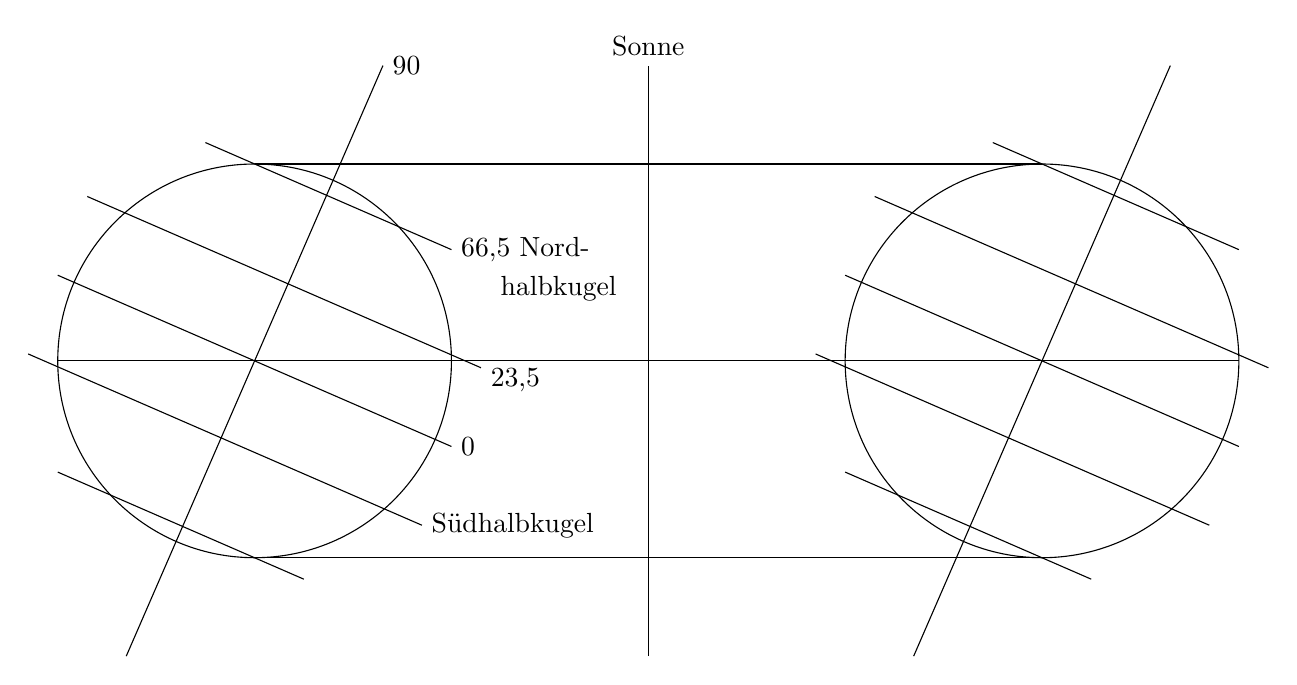
\begin{tikzpicture}[scale=2.5]
	\draw (-2,0) circle (1cm);				%% Linke Erde
	\draw (-2.652,-1.5) -- (-1.348,1.5) node[right] {\ang{90}};	%% -- (-2,0) --
	\draw (-2.25,1.109) -- (-1,0.565) node[right] {\ang{66,5} Nord-};
	\draw (-0.8,0.365) node[right] {halbkugel};
	\draw (-2.85,0.835) -- (-0.85,-0.035);
	\draw (-0.85,-0.1) node[right] {\ang{23,5}};
	\draw (-3,0.435) -- (-1,-0.435) node[right] {\ang{0}};		%% Äquator
	\draw (-3.15,0.035) -- (-1.15,-0.835) node[right] {Südhalbkugel};
	\draw (-3,-0.565) -- (-1.75,-1.109);
	\draw (2,0) circle (1cm);				%% Rechte Erde
	\draw (2.652,1.5) -- (1.348,-1.5);	%% -- (-2,0) --
	\draw (1.75,1.109) -- (3,0.565);
	\draw (1.15,0.835) -- (3.15,-0.035);
	\draw (1,0.435) -- (3,-0.435);		%% Äquator
	\draw (0.85,0.035) -- (2.85,-0.835);
	\draw (1,-0.565) -- (2.25,-1.109);
%%
	\draw (0,-1.5) -- (0,1.5) node[above] {Sonne};
	\draw (-3,0) -- (3,0);
	\draw (-2,-1) -- (2,-1);
	\draw (-2,1) -- (2,1);
%	\draw[fill=blue, thick] (-2,0) -- (66.5:1) arc (66.5:66.5:1);
  \end{tikzpicture}
  \captionof{figure}{Modell der Erde und ihrer Umlaufbahn um die Sonne}
\end{figurewrapper}

\newcommand{\Legendeitem}[2]{\begin{tikzpicture}\draw[color=Klimaguertel#1,fill] circle (0.15cm);\end{tikzpicture}
#2

}
\begin{landscape}
%\thispagestyle{empty}
\begin{figurewrapper}
	\includegraphics[width=1\hsize]{files/images/Klimaguertel-der-erde}
	\subsection*{Legende}
	\begin{minipage}{4cm}
	\begin{flushleft}
		\Legendeitem{Eisklima}{Eisklima}
		\Legendeitem{Tundrenklima}{Tundrenklima}
		\Legendeitem{Boreales}{Boreales Klima}
	\end{flushleft}
	\end{minipage}
	\begin{minipage}{5cm}
	\begin{flushleft}
		\Legendeitem{Warm}{Warmgemäßigtes Klima}
		\Legendeitem{Subtropisch}{Subtropisches Klima}
		\Legendeitem{Tropisch}{Tropisches Klima}
	\end{flushleft}
	\end{minipage}\hfill
	\begin{minipage}{13cm}
	Die Urheberrechte liegen bei LordToran
	\url{http://de.wikipedia.org/w/index.php?title=Datei:Klimagürtel-der-erde.svg&filetimestamp=20071015144227}
	\end{minipage}
	\captionof{figure}{Klimagürtel der Erde}
\end{figurewrapper}
\end{landscape}

\subsection{Kosmische Gegebenheiten}
\begin{itemize}
	\item Die Erde ist der dritte Planet im Sonnensystem (149 Millionen \si{\kilo\metre} von der Sonne entfernt)
	\item Die durchschnittliche Oberflächentemperatur liegt zwischen \SIrange{10}{20}{\celsius}
	  (Venus ist um 25\,\% näher an der Sonne:
	  Oberflächentemperatur: \SI{470}{\celsius}. Mars ist um 50\,\% weiter von der Sonne entfernt:
	  Oberflächentemperatur: \SIrange{-60}{60}{\celsius}).
	  Die Lage im Raum ist verantwortlich für das lebensfreundliche Klima.
	\item Sie bewegt sich auf einer elliptischen Bahn um die Sonne, die sich in einem Brennpunkt der Ellipse befindet.
	\item Die Erde dreht sich in knapp 24 Stunden einmal um ihre eigene Achse
	  (vor 400 Millionen Jahren betrug die Tageslänge 22 Stunden).
	\item Für einen Bahnumlauf benötigt die Erde 365 Tage (vor 400 Millionen Jahre 400 Tage).
	\item Die Rotationsachse der Erde um \ang{23,5} gegen die Ekliptik geneigt.
	\item Die Rotationsachse der Erde pendelt (circa \ang{0,5}), das heißt, sie beschreibt die Form eines Doppelkegels.
	  Für einen vollständigen Umlauf benötigt sie circa \numprint{26000} Jahre, ein sogenanntes platonisches Weltenjahr.
	\item Die Erde ähnelt einer an den Polen abgeflachten Kugel.
\end{itemize}

Erklären Sie folgende Phänomene:
\begin{description}
	\item[Tag-/Nachtwechsel:] Die Erde dreht sich in knapp 24 Stunden einmal um ihre Rotationsachse,
	  diese steht aber nicht ganz senkrecht zur Ekliptik. Die Sonne ist minütlich
	  über einem anderen Ort im Zenit und bescheint immer nur die halbe Kugel.
	\item[Jahreszeiten -- aber nicht überall:] Die Erdachse ist um \ang{23,5} gegen die Ekliptik geneigt und
	  sie bewegt sich auf einer elliptischen
	  Bahn um die Sonne. Dadurch ändert sich der Sonneneinfallswinkel und damit die einfallende Energiemenge pro \si{\metre\squared}
	  für jeden Ort. Wendekreis zu Wendekreis 100--90\,\%, Wendekreis zu Polarkreis 90--40\,\% und
	  Polarkreis zu Pol 40--0\,\%. Dadurch gibt es zwischen Wendekreis zu Polarkreis vier Jahreszeiten und
	  Polarkreis zu Pol zwei Jahreszeiten. Die elliptische Bahn der Erde, die circa 2 Millionen \si{\kilo\metre}
	  Entfernungsunterschied ausmacht, begünstigt die Nordhalbkugel noch indem hierdurch die Sommer kälter
	  (da weiter von der Sonne Entfernt) und die Winter wärmer werden als auf dem entsprechenden Breitengrad auf der
	  Südhalbkugel.
	\item[Abnahme der Tageslänge im Laufe der Jahre:] Die Erdachse beschreibt eine Pendelbewegung.
	  Dadurch ändert sich die Lade der Erdachse zur Sonne (circa \ang{2}). Für eine vollständige Pendelbewegung
	  braucht die Erde \numprint{26000} Jahre. Dadurch ändert sich der Sonneneinfallswinkel und
	  die Lage der Polarkreise $\rightarrow$ Eiszeiten
\end{description}

%\renewcommand{\longtableheader}{ & \rowcolor{blue} \textbf{Zone der Polarkappe} & \rowcolor{green} \textbf{Mittelgürtel}
%& \rowcolor{red!70} \textbf{Heißer Gürtel} \\}		%% \rowcolor wird nicht akzeptiert
\renewcommand{\longtableheader}{ & \textbf{Zone der Polarkappe} & \textbf{Mittelgürtel}
& \textbf{Heißer Gürtel} \\ \hline}
\begin{longtable}{L{2.2cm}|L{4cm}|L{4cm}|L{4cm}}
	\longtableheader
	\endfirsthead

	\longtableheader
	\endhead

	\caption{Eigenschaften von Wendekreis, Polarkreis und der Pole}
	\endlastfoot

	\multicolumn{4}{r}{\longtableendfoot} \\
	\endfoot

	\textbf{Lage}						& Pol bis Polarkreis \ang{90}--\ang{66,5}		& Polarkreis bis Wendekreis (\ang{66,5}--\ang{23,5})
	  & Wendekreis bis Wendekreis (\ang{23,5}--\ang{0})\\ \hline
	\textbf{Tag/Nacht Verhältnis}		& circa \nicefrac{1}{2} Jahre, Tag (24:0) und \nicefrac{1}{2} Jahr Nacht (0:24)
	  & Variabler Jahreslauf, Balingen: 16:8 bzw. 8:16		& durchgehend circa 12:12 (\SI{+- 1,5}{\hour})\\ \hline
	\textbf{Jahres\-zeiten}				& zwei Polartag und Polarnacht		& Vier Winter N>T, Sommer T>N % zwei Übergänge
	  & Keine\\ \hline
	\textbf{\nicefrac{Energie}{\si{\metre\squared}}}& circa 20\,\%		& circa 70\,\%	& circa 95\,\%\\ \hline
	\textbf{Klimatyp}					& 2 Jahreszeiten	& 4 Jahreszeiten& Tageszeitenklima\\
\end{longtable}

\subsection{Vom Klimadiagramm zur Klimazone}
Für die Produktion im primären Wirtschaftssektor spielen die klimatischen Faktoren eine herausragende Rolle.
Der primäre Wirtschaftssektor ist auch die Basis für die Ernährung der Bevölkerung.
Klimatische Faktoren entscheiden also wie effektiv an einem bestimmten Ort \fxwarning{Quelle unleserlich}
Wirtschaft betrieben werden kann (Überleben/Überschüsse).

Neben der eingestrahlten Energiemenge pro \si{\metre\squared} beeinflussen noch folgende Faktoren das lokale Klima:

\begin{itemize}
	\item Mensch (antropogene Einflüsse, Schadstoffe; Treibhauseffekt)
	\item Höhenlage (\SI{100}{\meter} $\rightarrow$ \ang{0,65})
	\item Meeresströmung
	\item Vegetation, Bodenverhältnisse
	\item Relief (Gebirge, Ebene)
\end{itemize}

\subsection{Wie erfasst man das Klima?}
\begin{eqlist}
	\item[Langfristig:] Beschreibung der Vegetation
	\item[Kurzfristig:] Temperatur und Niederschlag
\end{eqlist}


\subsection{Klimadiagramme}
\ifDraft{
Klimadiagramme zu Stuttgart-Schnarrenberg: Siehe Anhang
}{}
\newcommand{\UrheberrechteText}{\hfill Grafik kann aufgrund von Urheberrechten hier nicht abgebildet werden.}

\newcommand{\scaleKlimadiagramme}{\hsize}
\newcommand{\KlimadiagrammeOrt}{Amundsen Scott/USA}
\subsubsection{\KlimadiagrammeOrt}
\ifDraft{%
\begin{figurewrapper}
	\includegraphics[width=\scaleKlimadiagramme]{files/images/Klimadiagramme/1}
	\captionof{figure}{Klimadiagramm: \KlimadiagrammeOrt}
\end{figurewrapper}}{\UrheberrechteText}

\begin{description}
	\item[Lage:] \SI{2800}{\meter} über dem Meeresspiegel, Südpol, südlich von Greenwich $\rightarrow$ \ang{90;00;}\,S, \ang{00;00;}\,O
	\item[Temperaturverlauf:] Juli, August und September sind mit \SI{-60}{\celsius} die kühlsten Monate,
		während Dezember und Januar mit knapp unter \SI{-30}{\celsius} die vergleichsweise \enquote{wärmsten} sind.
		Ab Januar sinkt die Temperatur bis Juli und ab September steigt sie bis Dezember $\rightarrow$ Permafrost.

		Es ist also durchweg extrem kalt: Durchschnittstemperatur im Jahr: \SI{-49,3}{\celsius}
	\item[Niederschlagsverlauf:] Kein Niederschlag
	\item[Klima-/Vegetationszone:] Keine Vegetation, Zone der Polarkappen, 2 Jahreszeitenklima, Polare Zone
	\item[Landwirtschaft:] Keine -- maximal Fischfang möglich
\end{description}

\renewcommand{\KlimadiagrammeOrt}{Chatanga/Russland}
\subsubsection{\KlimadiagrammeOrt}
\ifDraft{%
\begin{figurewrapper}
	\includegraphics[width=\scaleKlimadiagramme]{files/images/Klimadiagramme/2}
	\captionof{figure}{Klimadiagramm: \KlimadiagrammeOrt}
\end{figurewrapper}}{\UrheberrechteText}

\begin{description}
	\item[Lage:] \SI{33}{\meter} über dem Meeresspiegel, Nordhalbkugel, \ang{71;59;}\,S, \ang{102;28;}\,O
	\item[Temperaturverlauf:] Juli ist mit über \SI{10}{\celsius} der wärmste Monat (kühler Sommer),
		während der Januar mit \SI{-35}{\celsius} der kälteste ist (Winter extrem kalt).
		Von Januar steigt die Temperatur kontinuierlich bis Juli, dann fällt sie wieder $\rightarrow$ Permafrost.
	\item[Niederschlagsverlauf:]  Im September gibt es mit über \SI{30}{\milli\meter} den meisten Niederschlag,
		während es im Januar und Februar mit knapp über \SI{10}{\milli\meter} nur sehr wenig regnet.
		Vom Januar bis zum Mai liegt der Niederschlag zwischen 10 und \SI{20}{\milli\meter}.
		Vom Juni bis zum Dezember liegt der Niederschlag zwischen 20 und \SI{35}{\milli\meter}
		mit abnehmender Tendenz nach September $\rightarrow$ humide Monate aber insgesamt trocken.

		\nicefrac{Gesamtniederschlag}{Jahr} = \SI{270,1}{\milli\meter}
	\item[Klima-/Vegetationszone:] Keine mehrjährigen Pflanzen, Zone der Polkappen, subpolare Zone, 2/4 Jahreszeitenklima
	\item[Landwirtschaft:] Fischfang, Viehzucht (Rentiere)

		(nomadisierend) $\rightarrow$ Rohstoffabbau
\end{description}

\renewcommand{\KlimadiagrammeOrt}{Novgorod/Russland}
\subsubsection{\KlimadiagrammeOrt}
\ifDraft{%
\begin{figurewrapper}
	\includegraphics[width=\scaleKlimadiagramme]{files/images/Klimadiagramme/3}
	\captionof{figure}{Klimadiagramm: \KlimadiagrammeOrt}
\end{figurewrapper}}{\UrheberrechteText}

\begin{description}
	\item[Lage:] \SI{24}{\meter} über dem Meeresspiegel, Nordhalbkugel, \ang{58;31;}\,S, \ang{31;15;}\,O
	\item[Temperaturverlauf:] Juli ist mir über \SI{15}{\celsius} der wärmste der Klimazone, während Januar und Februar
		mit knapp \SI{-10}{\celsius} die kälteste bis extrem kalten sind. Ab Februar steigt die Temperatur bis Juli,
		dann sinkt sie wieder.
		\begin{itemize}
			\item Durchschnittstemperatur im Jahr: \SI{4,3}{\celsius}
		\end{itemize}
	\item[Niederschlagsverlauf:] Im Juli und August regnet es am meisten (über \SI{65}{\milli\meter}),
		während der Februar mit einem Niederschlag von circa \SI{20}{\milli\meter} der Niederschlagsärmste ist.
		Von Februar nimmt der Niederschlag bis Juli/August kontinuierlich zu und von August bis Februar ebenso ab.
		$\rightarrow$ Es sid alles humide Monate

		\nicefrac{Gesamtniederschlag}{Jahr} = \SI{558}{\milli\meter}
	\item[Klima-/Vegetationszone:] Mittelgürtel, kalt gemäßigte Zone, 4 Jahreszeitenklima
	\item[Landwirtschaft:] Forstwirtschaft (boreale Wälder-Taiga), Anbau von Sommergerste, Rentiernomaden
\end{description}

\renewcommand{\KlimadiagrammeOrt}{Aachen}
\subsubsection{\KlimadiagrammeOrt}
\ifDraft{%
\begin{figurewrapper}
	\includegraphics[width=\scaleKlimadiagramme]{files/images/Klimadiagramme/4}
	\captionof{figure}{Klimadiagramm: \KlimadiagrammeOrt}
\end{figurewrapper}}{\UrheberrechteText}

\begin{description}
	\item[Lage:] \SI{202}{\meter} über dem Meeresspiegel, Nordhalbkugel, \ang{50;47;}\,S, \ang{06;06;}\,O
	\item[Temperaturverlauf:]
		\begin{itemize}
			\item Kälteste Monate: Januar, Februar, Dezember mit circa \SI{5}{\celsius}
			\item Wärmste Monate: Juni, Juli, August mit \SIrange{15}{20}{\celsius}
			\item Durchschnittstemperatur im Jahr: \SI{10}{\celsius}
			\begin{itemize}
				\item insgesamt kühl, warme Sommer -- kalte Winter, mehr als 120 Tage über \SI{10}{\celsius}
			\end{itemize}
		\end{itemize}
	\item[Niederschlagsverlauf:] ziemlich konstant $\rightarrow$ humide Zone

		\nicefrac{Gesamtniederschlag}{Jahr} = \SI{807}{\milli\meter}
	\item[Klima-/Vegetationszone:] 4 Jahreszeitenklima, Mittelgürtel, kühl gemäßigte Zone
	\item[Landwirtschaft:] Weidewirtschaft, Viehzucht, Milchwirtschaft,
		Ackerbau (Getreide, Hülsenfrüchte, Kartoffeln, Zuckerrüben), Forstwirtschaft
\end{description}

\renewcommand{\KlimadiagrammeOrt}{Soci/Russland}
\subsubsection{\KlimadiagrammeOrt}
\label{subsubsec:Klimadiagramme:Soci:Russland}
\ifDraft{%
\begin{figurewrapper}
	\includegraphics[width=\scaleKlimadiagramme]{files/images/Klimadiagramme/5}
	\captionof{figure}{Klimadiagramm: \KlimadiagrammeOrt}
\end{figurewrapper}}{\UrheberrechteText}

\begin{description}
	\item[Lage:] \SI{34}{\meter} über dem Meeresspiegel, Nordhalbkugel, \ang{43;35;}\,S, \ang{39;46;}\,O
	\item[Temperaturverlauf:]
		\begin{itemize}
			\item Kälteste Monate: Januar, Februar, Dezember mit circa \SI{5}{\celsius}
			\item Wärmste Monate: Juni, Juli, August mit \SIrange{20}{25}{\celsius}
			\item Durchschnittstemperatur im Jahr: \SI{14}{\celsius}
			\begin{itemize}
				\item kühle Winter -- heiße Sommergerste
				\item Insgesamt warm, ganz jährig feucht, kein Frost
			\end{itemize}
		\end{itemize}
	\item[Niederschlagsverlauf:] Konstante Niederschlagsmenge

		\nicefrac{Gesamtniederschlag}{Jahr} = \SI{1571,7}{\milli\meter}
	\item[Klima-/Vegetationszone:] 4 Jahreszeitenklima, Mittelgürtel, immerfeuchte Subtropen
	\item[Landwirtschaft:] Weinwirtschaft, Forstwirtschaft, Getreideanbau, Mandeln, Feigen, Tee, Oliven,
		Zitrusfrüchte, Tabak, Baumwolle, Erdnüsse, Wein \fxwarning{Weinwirtschaft ???}
\end{description}

\newcommand{\scaleKlimadiagrammetwo}{0.7\hsize}
\renewcommand{\KlimadiagrammeOrt}{Palermo/Italien}
\subsubsection{\KlimadiagrammeOrt}
\ifDraft{%
\begin{figurewrapper}
	\includegraphics[width=\scaleKlimadiagrammetwo]{files/images/Klimadiagramme/6}
	\captionof{figure}{Klimadiagramm: \KlimadiagrammeOrt}
\end{figurewrapper}}{\UrheberrechteText}

\begin{description}
	\item[Lage:] \SI{21}{\meter} über dem Meeresspiegel, Nordhalbkugel
	\item[Temperaturverlauf:] Insgesamt warm kühle, feuchte Winter und heiße, trockene Sommer
	\item[Niederschlagsverlauf:] Winterregen, Sommer nur wenig
	\item[Klima-/Vegetationszone:] 4 Jahreszeitenklima, Mittelgürtel, wechsel-feuchte Subtropen
	\item[Landwirtschaft:] \SieheC{subsubsec:Klimadiagramme:Soci:Russland}{Soci/Russland}
\end{description}

\renewcommand{\KlimadiagrammeOrt}{Sebha/Libyen}
\subsubsection{\KlimadiagrammeOrt}
\label{subsubsec:Klimadiagramme:Sebha:Libyen}
\ifDraft{%
\begin{figurewrapper}
	\includegraphics[width=\scaleKlimadiagrammetwo]{files/images/Klimadiagramme/7}
	\captionof{figure}{Klimadiagramm: \KlimadiagrammeOrt}
\end{figurewrapper}}{\UrheberrechteText}

\begin{description}
	\item[Lage:] Nordhalbkugel, heiße Sommer und warme Winter, insgesamt sehr trocken- arid
	\item[Klima-/Vegetationszone:] 4 Jahreszeitenklima, Mittelgürtel, trockene Subtropen
	\item[Landwirtschaft:] Nomaden mit Viehwirtschaft (je nach Trockenheit von Rind über Schaf zu Ziege)
		Oasenwirtschaft, Bewässerungsanbau (Datteln und Ölbäume)
\end{description}

\renewcommand{\KlimadiagrammeOrt}{Timbuktu/Mali}
\subsubsection{\KlimadiagrammeOrt}
\ifDraft{%
\begin{figurewrapper}
	\includegraphics[width=\scaleKlimadiagrammetwo]{files/images/Klimadiagramme/8}
	\captionof{figure}{Klimadiagramm: \KlimadiagrammeOrt}
\end{figurewrapper}}{\UrheberrechteText}

\begin{description}
	\item[Lage:] Nordhalbkugel, ganzjährig heiß, nurgeringe Schwankungen (\SI{8}{\celsius}),
		nur im Nordsommer für einen Monat feucht, sonst sehr trocken, Sommerregen, (semi-)arid
	\item[Klima-/Vegetationszone:] 4 Jahreszeitenklima, heißer Gürtel, trockene Subtropen bis Tropen
	\item[Landwirtschaft:] \SieheC{subsubsec:Klimadiagramme:Sebha:Libyen}{Sebha/Libyen}
\end{description}

\renewcommand{\KlimadiagrammeOrt}{Moanda/Gabun}
\subsubsection{\KlimadiagrammeOrt}
\ifDraft{%
\begin{figurewrapper}
	\includegraphics[width=\scaleKlimadiagrammetwo]{files/images/Klimadiagramme/9}
	\captionof{figure}{Klimadiagramm: \KlimadiagrammeOrt}
\end{figurewrapper}}{\UrheberrechteText}

\begin{description}
	\item[Lage:] Am Äquator, ganzjährig warm/heiß, nur geringe Schwankungen, im Nordsommer sehr trocken,
		im Nordwinter feucht (Winterregen, Regenzeit) insgesamt Feucht
	\item[Klima-/Vegetationszone:] Tageszeitenklima, heiser Gürtel, wechselfeuchte Tropen
	\item[Landwirtschaft:] Regenfeldanbau (Reis, zwei Ernten pro Jahr) Plantagen
		(Erdnüsse, Baumwolle, Mais, Yamswurzel, Maniok) zunehmend Forstwirtschaft
\end{description}

\renewcommand{\KlimadiagrammeOrt}{Belem/Brasilien}
\subsubsection{\KlimadiagrammeOrt}
\ifDraft{%
\begin{figurewrapper}
	\includegraphics[width=\scaleKlimadiagrammetwo]{files/images/Klimadiagramme/10}
	\captionof{figure}{Klimadiagramm: \KlimadiagrammeOrt}
\end{figurewrapper}}{\UrheberrechteText}

\begin{description}
	\item[Lage:] Südhalbkugel, ganzjährig heiß, insgesamt extrem feucht, immer humid
	\item[Klima-/Vegetationszone:] Tageszeitenklima, heiser Gürtel, immerfeuchte Tropen
	\item[Landwirtschaft:] Forstwirtschaft, Waldnutzung (Gummi, Gerbstoffe, Harze), Wanderfeldbau
		zum Teil Dauerfeldbau in China und Thailand. Plantagen: Kantschuk, Banane
\end{description}

\subsection{Ergebnisse der Klimazonenarbeit}
\begin{itemize}
	\item Die einzelnen Klimazonen sind unterschiedlich gut nutzbar.
	\item Die gemäßigte, wechselfeuchte und immerfeuchte Zonen können Überschüsse an Nahrungsmittel produzieren.
	  Aufgrund der Landmassenverteilung kommen diese Gebiete fast ausschließlich auf der Nordhalbkugel vor.
	\item Die reichsten Länder dieser Welt (traditionell) konzentrieren sich auf die Nordhalbkugel.
	\item Ist der primäre Wirtschaftssektor verantwortlich für diesen Reichtum?
\end{itemize}
